\subsection{Geschwindigkeit}
\label{ssec:evaluation:messungen:geschwindigkeit}
%In diesem Abschnitt soll untersucht werden, ob eine Reduzierung der Geschwindigkeit positive Auswirkungen auf die Zuverlässigkeit von Bildverarbeitung und Regelung besitzt.

Nachdem eine passende Einstellung der Regel-und Bildverarbeitungsfrequenz gefunden wurde, soll nun das Fahren mit höheren Geschwindigkeiten betrachtet werden. Neben der Sichtprüfung der Funktionalität der Fahrspurverfolgung wurden die Anzahl der zur Zielpunktbestimmung genutzten Punkte pro Regelungsiteration und der prozentuale Anteil an nicht bestimmten Zielpunkten zur Untersuchung herangezogen. 

Zur besseren Vergleichbarkeit der Messergebnisse wurden die Daten für je eine entgegen des Uhrzeigersinnes gefahrene Runde mit \SI{3}{\hertz} Bildverarbeitungsfrequenz aufgenommen.

Abbildung~\ref{fig:evaluation:riverflow:regelungspunkte:je_linie} zeigt exemplarisch für die Geschwindigkeit \( \gls{lat:velocity} = 
\SI{0,2}{\metre\per\second} \) die  Anzahl jeweiliger Linienpunkttypen zur Zielpunktberechnung. Es fällt sogleich auf, dass die Mittellinie einen kleineren Einfluss nimmt. Da pro Strich und Bild nur ein Punkt in der Weltkarte 
eingetragen wird, ist deren Punkteanzahl geringer. Wie unter 
\ref{item:regelung:zielpunkt:holen:regeln:xcoord} in Kapitel 
\ref{ssec:regelung:zielpunkt:holen} beschrieben, werden die Regelungspunkte unter anderem nach ihrer x-Koordinate ausgewählt. In einer Linkskurve fallen dadurch mehr Punkte der linken Randlinie in das Suchfenster. Da die Strecke in 
der befahrenen Richtung vorrangig Linkskurven aufweist, werden im Mittel mehr linke als rechte Randpunkte zur Zielpunktberechnung herangezogen.

\begin{figure}[htbp] % [htb]
	\centering
	\subfloat[Anzahl der jeweiligen zur Regelung genutzten Punkte aus der Weltkarte bei \( \gls{lat:velocity} = \SI{0,2}{\metre\per\second} \) 
	\label{fig:evaluation:riverflow:regelungspunkte:je_linie}]{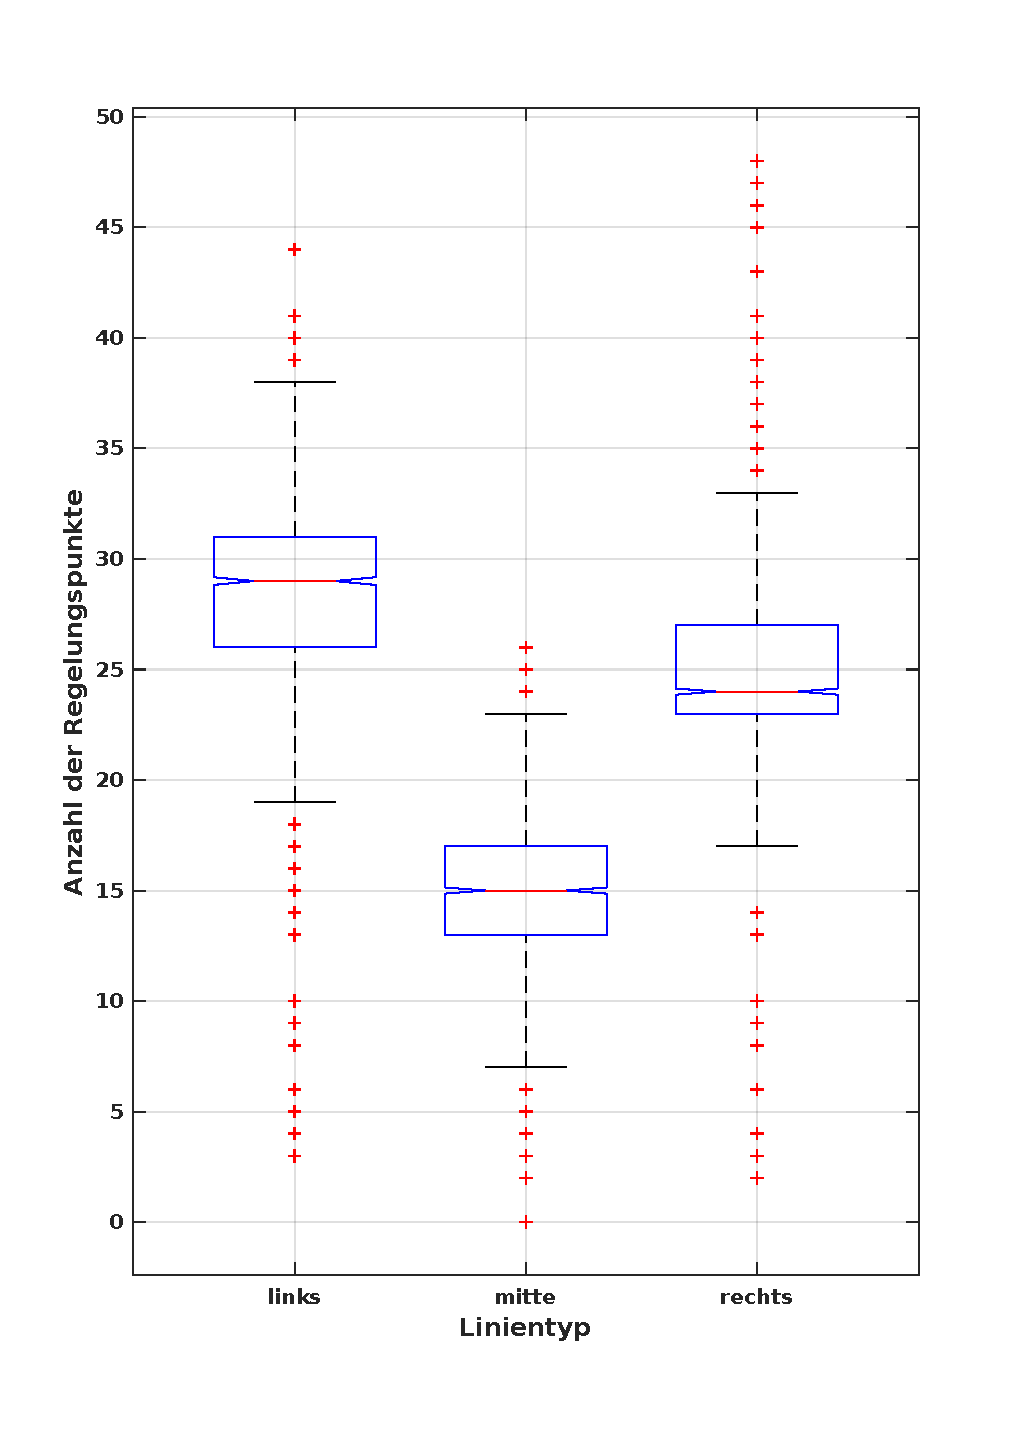
\includegraphics[height=0.35\textheight]{evaluation_riverflow_regelungspunkte_je_linie_0_2m_s_3Hz.pdf}}
	\hfill
	\subfloat[Anzahl der zur Regelung verwendeten Kartenpunkte zu verschiedenen 
	Geschwindigkeiten
	\label{fig:evaluation:riverflow:regelungspunkte:je_geschw}]{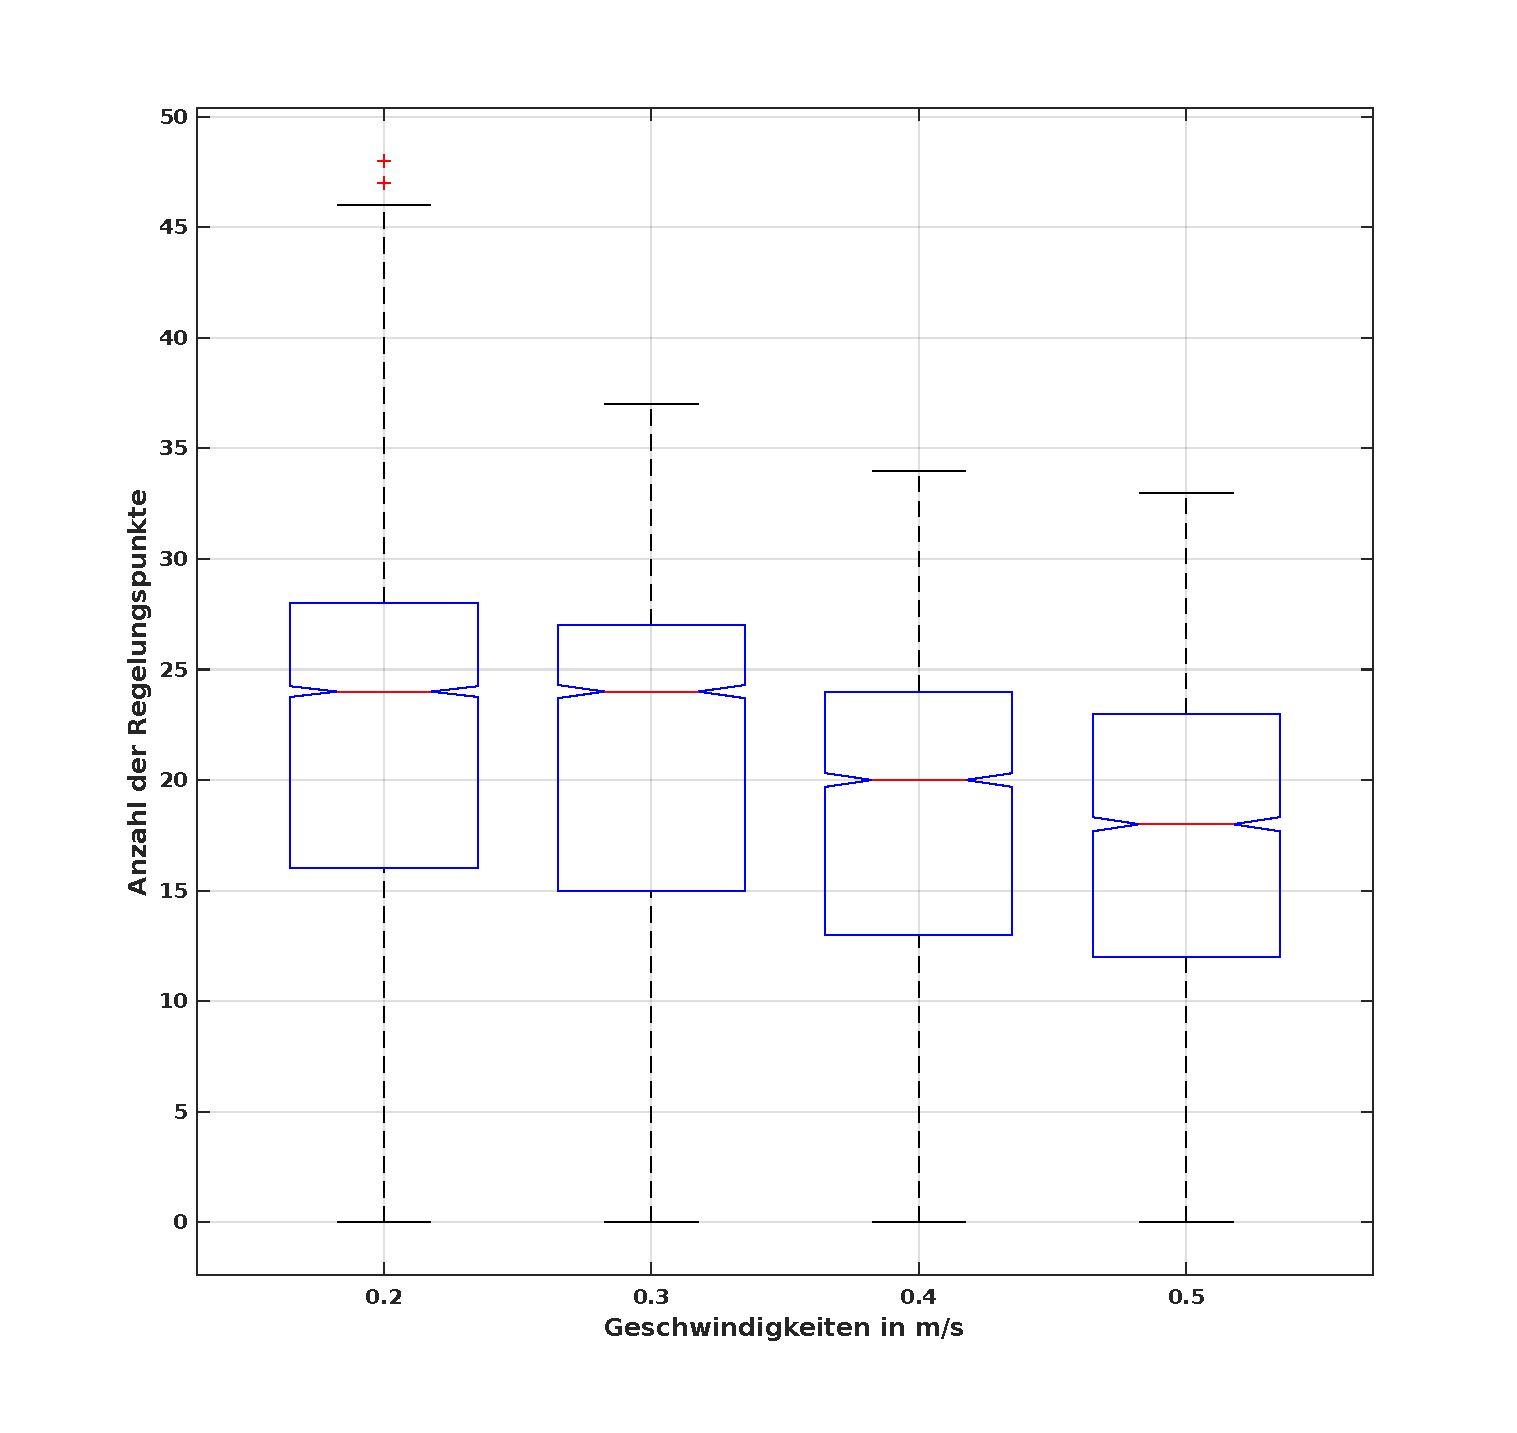
\includegraphics[height=0.35\textheight]{evaluation_riverflow_regelungspunkte_je_geschw_3Hz.pdf}}
	\caption{Boxplots zur Menge der Punkte, welche in einem Regelungsintervall 
	aus der Weltkarte entnommen und zur Zielpunktberechnung verwendet werden}
	\label{fig:evaluation:riverflow:regelungspunkte}
\end{figure}

Betrachten wir die Gesamtzahl der zur Regelung verwendeten Punkte, ist wie in 
Abbildung~\ref{fig:evaluation:riverflow:regelungspunkte:je_geschw} ein Abfallen der Anzahl mit ansteigender Geschwindigkeit des Fahrzeugs zu beobachten. Wenn das Auto schneller fährt, liegt ein Punkt in der Karte umso eher außerhalb des Bereiches, aus dem die Regelungspunkte genutzt werden. Bei gleichbleibender Bildfrequenz wird zwischen jedem Bild eine größere Strecke zurückgelegt, sodass die Dichte der Weltkartenpunkte geringer wird. Der dargestellte Boxplot erfüllt also die Erwartungen.

Die mit unserer Implementierung erreichbare Höchstgeschwindigkeit sollte folglich dann erreicht sein, wenn der mobile Roboter fast ausschließlich nach den Informationen eines Bildes regelt oder sogar zwischenzeitlich keine Zielpunkte mangels Regelungspunkten bestimmen kann. Mit anderen Worten: Wenn sich das Auto zwischen zwei Aufnahmen bis zum Sichtende des ersten Bildes bewegt, wie der Riverflow-Algorithmus Punkte erkennen konnte, ist die Maximalgeschwindigkeit beinahe erreicht. Ein Indiz dafür ist neben der visuellen Auffälligkeit des Fahrspurverlasses die starke Zunahme der nicht gefundenen Zielpunkte. 

\begin{figure}[htbp] % [htb]
	\centering
	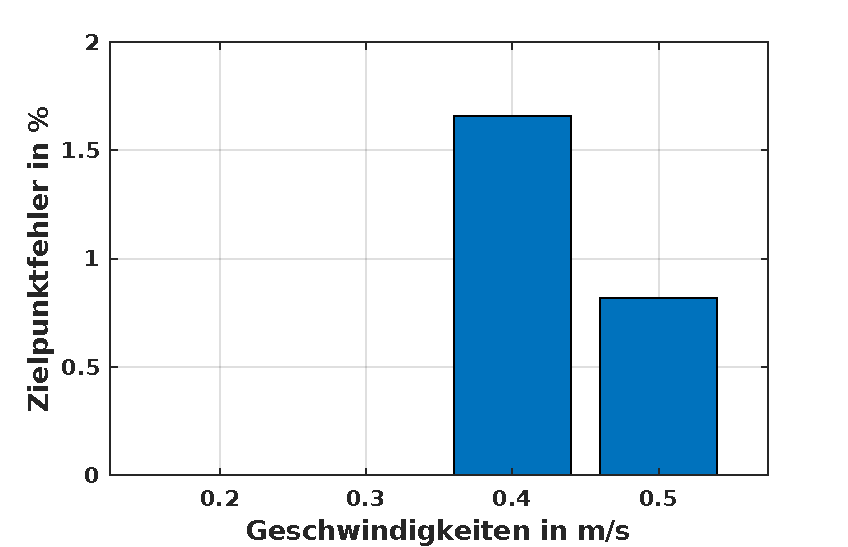
\includegraphics[width=0.7\textwidth]{evaluation_riverflow_zielpunktfehler_je_geschw_3Hz.pdf}
	\caption{Anteil der unbestimmten Zielpunkte einer Runde auf dem Parcours mit verschiedenen Geschwindigkeiten}
	\label{fig:evaluation:riverflow:zielpunktfehler_je_geschw}
\end{figure}

Was in Abbildung~\ref{fig:evaluation:riverflow:zielpunktfehler_je_geschw} zu sehen ist, war ebenfalls während des Fahrversuches am Auto zu beobachten. Ab einer Geschwindigkeit von \( \gls{lat:velocity} = \SI{0,4}{\metre\per\second} \) fuhr das Fahrzeug instabiler und die Latenzzeit der Regelung war dahingehend zu bemerken, dass in Kurven meist etwas zu spät und kurz darauf zur Korrektur zu viel eingelenkt wurde. Dies führte zu einer schwingenden Fahrweise (das Auto fuhr \glqq Schlängellinien\grqq). 

Die begrenzende Komponente für die Geschwindigkeit ist hier neben der Bildfrequenz allerdings auch das Getriebe. Durch dessen kurze Übersetzung beträgt die Geschwindigkeit im Maximum 4500 tics pro Sekunde, was in etwa \SI{0,43}{\metre\per\second} entspricht. Die im Plot bezeichneten \SI{0,5}{\metre\per\second} dürften folglich nicht genau stimmen, auch wenn dies der eingestellte Wert des Geschwindigkeitsparameters war. Sie geben die Daten zu der dem ersten Auto maximal physikalisch möglichen Geschwindigkeit an. 

Ergänzend muss hier erwähnt werden, dass bereits ein zweites Fahrzeug mit ca. doppelt so langer Übersetzung existiert. Jedoch misslang eine Testfahrt mit unveränderten Parametereinstellungen bei höheren Geschwindigkeiten. Auch hier zeigte sich die Grenze an der \SI{0,5}{\metre\per\second}-Marke.

Dass diese Geschwindigkeit auch die Grenze der Stabilität des Algorithmus war, zeigte ein \glqq Dauertest\grqq{} von zehn Runden. Bis zu einer Geschwindigkeit von \SI{0,3}{\metre\per\second} führte der Versuch zu keinen nennenswerten Problemen in der Fahrspurverfolgung. Auch wenn während der schnelleren \SI{0,4}{\metre\per\second}-Fahrt zehn Runden erfolgreich abgefahren wurden, kam hier das Fahrzeug mitunter stark ins Schwingen und befand sich kurz davor, den Fahrstreifen zu verlieren. Mit der höchstmöglichen Geschwindigkeit wurde der Dauertest nicht bestanden, da das Auto schon nach zwei Runden von der Straße abkam.